\documentclass[10pt]{article}
\usepackage{commands}


\begin{document}
\begin{tcolorbox}
  \begin{center}
  \begin{Large}
    \textbf{PHYS 402 (Applications of Quantum Mechanics) Notes} \\
    \vspace{5pt}
  \end{Large}
  \begin{large}
        Rio Weil \\
\vspace{5pt}
    \emph{This document was typeset on \today}
  \end{large}
  \end{center}
\end{tcolorbox}

\begin{center}
  \textbf{Introduction:}

  This set of notes is based on UBC's PHYS 402 (Applications of Quantum Mechanics) course, taught by Dr. Robert Raussendorf. The course covers portions of the first five chapters of Sakurai's ``Modern Quantum Mechanics'', as well as some additional topics. If any errors are found in the notes, feel free to email me at \href{mailto:ryoweil6@student.ubc.ca}{ryoweil6@student.ubc.ca}.

\end{center}
\addtocontents{toc}{\protect\hypertarget{toc}{}}
\tableofcontents

\newpage
\section[Fundamental Concepts]{\hyperlink{toc}{Fundamental Concepts}}
\subsection{The beginnings of quantum mechanics}
Before we dive headfirst into the formalism of quantum mechanics, let us first review the first steps of the field as taken in the early 1900s. 

Our first founder is Max Planck; the problem at hand was the problem of the blackbody radiation spectrum. The two pre-existing laws (derived from thermodynamics arguments alone) predicting the BBR intensity as a function of frequency were flawed. The first was Wien's law (1896):
\begin{equation}
    I_{\text{Wien}}(f, T) \sim f^3\exp(-\frac{f}{T})
\end{equation}
which agreed with high frequency data well but failed to accurately describe low frequency emission. The second was Rayleigh-Jeans' law (1900):
\begin{equation}
    I_{\text{RJ}}(f, T) \sim f^4 T
\end{equation}
which agreed with low frequency data well but failed to accurately describe high frequency emission\footnote{It should be noted however that a full-derivation of the Rayleigh-Jeans law did not occur until 1905, at which point Planck had already established the more correct explanation.}. In fact, the intensity as predicted by Rayleigh-Jeans' diverges at high $\nu$, leading to the (obviously) erroneous conclusion that the total energy emitted by a black body is infinite; the so-called ``ultraviolet catastrophe''.

In order to solve this problem, in 1900 Planck proposed a quantum hypothesis; that light carries energy in individual packets, or quanta. In particular, for light of frequency $f$, each quanta carries energy:
\begin{equation}
    E = hf.
\end{equation}
Combining this quantum hypothesis with the Boltzmann supression of high-energy states (from thermodynamics), Planck's law was then derived to be:
\begin{equation}
    I_{\text{Planck}}(f, T) = \frac{2hf^3}{c^2}\frac{1}{\exp(\frac{hf}{k_B T}) - 1}
\end{equation}
which agrees with the BBR spectrum data across all frequencies\footnote{Further, we can observe that Planck's law agrees with Wien's law in the high-frequency limit, and with Rayleigh-Jeans' law in the low-frequency limit.}. It should also be noted that the integral over all $f$ of the above radiance law yields is finite, resolving the ultraviolet catastrophe. 

\begin{figure}[htbp]
    \centering
    TODO - plot of the three laws.
    \caption{<caption>}
    \label{fig-BBRspectra}
\end{figure}


\noindent
In the above discussion, we have introduced Planck's constant. It has numerical value\footnote{which is the set/absolute (rather than measured) value of the Planck constant as per the 2018 redefinition of SI units.}:
\begin{equation}
    h = 6.626070040 \times 10^{-34}\si{J.s}
\end{equation}
$h$ is quantified as ``small''. What exactly does small mean in this context? For comparison, $1\si{eV}$ is the kinetic energy of an electron acquired in a voltage drop of a Volt, $0.035\si{eV}$ is the average kinetic energy of an atom at room temperature (from $E_k = \frac{3}{2}k_B T$) and $2.4\si{eV}$ is the energy of a single photon from the middle of the visible spectrum ($600 \si{THz}$). The energy of a single photon, which depends on $h$, is in other words ``typical'' of microscopic phenomena.

Planck's quantum hypothesis would be confirmed in Einstein's (Nobel-prize winning) 1905 explanation of the photoelectric effect (which you likely covered in detail in a previous course in modern physics); namely that quanta of light transfer energy $E = hf$ to electrons in the metal, kicking them out\footnote{Provided of course that $hf > \Phi$ where $\Phi$ is the ``work function'' of the metal.}.

Our second founder of interest is DeBroglie. In 1924, he postulated that matter could behave like a wave, positing the DeBroglie wavelength relation:
\begin{equation}
    p = \frac{h}{\lambda}.
\end{equation}
The so-called ``wave-particle'' duality would be confirmed in 1927 by the Davisson-Germer experiment, which saw peaks of electron intensity at distinct angles, showing that electrons scatter in the same nature as photons.

Our third founder of interest is Schr\"{o}dinger, who postulated the Schr\"{o}dinger equation (expressed below in the position basis) in 1926:
\begin{equation}
    i\hbar \dpd{}{t}\Psi(\v{r}, t) = \left[\frac{-\hbar^2}{2m}\nabla^2 + V(\v{r}, t)\right] \Psi(\v{r}, t).
\end{equation}
It should be noted that this is one of the two core formulas of non-relativistic quantum mechanics, and is the quantum-mechanical equivalent of Newton's laws. It however does not cover the effects of special relativity (for which we defer the reader to a future course on quantum field theory) or quantum measurement (which we shall address now). 

An illuminating demonstration of quantum measurement takes the form of the Stern-Gerlach experiment (first carried out in 1921/1922; see \href{https://physicstoday.scitation.org/doi/10.1063/1.1650229}{this article} for more historical background). In this experiment, silver atoms are heated and escape from an oven with uniform velocity. The beam of atoms then pass through an inhomogenous magnetic field (generated by an asymmetric pair of magnetic pole pieces) where they are deflected, before hitting a screen where their position is recorded. 

\begin{figure}[htbp]
    \centering
    TODO - Sketch of the experiment
    \caption{Illustration of the Stern-Gerlach experiment.}
    \label{fig-SGexpsketch}
\end{figure}

Why are silver atoms used for this experiment? Moreover, what exactly is being measured? For this, we consider a simplified model of the atom (which will suffice for the purposes of explaining this experiment). Silver atoms consist of 47 electrons in the shell, and 47 protons and 61 neutrons in the nucleus. A first guess of the mechanism of the atoms being deflected by the magnetic field may be a Lorentz force effect; however this is not the case as the atoms are electrically neutral. Instead, the silver atom has a single unpaired electron which has an intrinsic angular momentum, known as spin. In particular, the electron is spin-1/2\footnote{We will return to a more detailed discussion of angular momentum and spin at a later portion of the course}. This provides the silver atom with a net magnetic moment $\gv{\mu}$ proportional to the electron spin\footnote{The astute reader may question why the spin of the unpaired proton in the nucleus has no contribution to the net magnetic moment. This is due to the fact that the proportionality factor between the spin and magnetic moment has a factor of inverse mass. Since the proton is 1836 times heavier than the electron, the proton's magnetic moment contribution is negligeble compared to the electron's.} $\v{S}$:

\begin{equation}
    \gv{\mu} \propto \v{S}.
\end{equation}
We then recall from electromagnetism that a magnetic dipole $\gv{\mu}$ in a magnetic field $\v{B}$ has interaction energy:
\begin{equation}
    E = -\gv{\mu} \cdot \v{B}.
\end{equation}
We can then find the force that the dipole feels by taking the (negative) gradient of the energy:
\begin{equation}
    \v{F} = -\gv{\nabla}(-\gv{\mu} \cdot \v{B}) = \mat{\dpd{}{x}(\gv{\mu} \cdot \v{B}) \\ \dpd{}{y}(\gv{\mu} \cdot \v{B}) \\ \dpd{}{z}(\gv{\mu} \cdot \v{B})}.
\end{equation}
Ignoring the magnetic fields that are not in the $z$-direction, we find the force on the silver atoms in the $z$-direction to be:
\begin{equation}
    F_z = \mu_z \dpd{B_z}{z}.
\end{equation}
So in the inhomogenous field produced by the asymmetric magnets, the silver atoms should feel an up/downwards force depending on the direction of $\v{S}$ (which determines $\mu_z$). 

\begin{figure}[htbp]
    \centering
    TODO - Picture
    \caption{The inhomogenous magnetic field used in the Stern-Gerlach experiment, which deflects the silver atoms due to their magnetic dipole moment proportional to electron spin.}
    \label{fig-SGexpmagnet}
\end{figure}

Classically, the magnetic moment $\v{\mu}$ can point in any direction, and therefore $\mu_z$ ranges continuously from $+\abs{\gv{\mu}}$ to $-\abs{\gv{\mu}}$. Hence, the signature we would expect on the Stern-Gerlach experiment screen (wherein the vertical position of the atoms on the screen corresponds to a measurement of the $z$-component of the magnetic moment) would be a continuous band, as seen in the left of Fig. 1.4 below. However, this is \emph{not} what is observed; instead the experimental result was two discrete dots with nothing in between, as seen in the right of the figure. 

\begin{figure}[htbp]
    \centering
    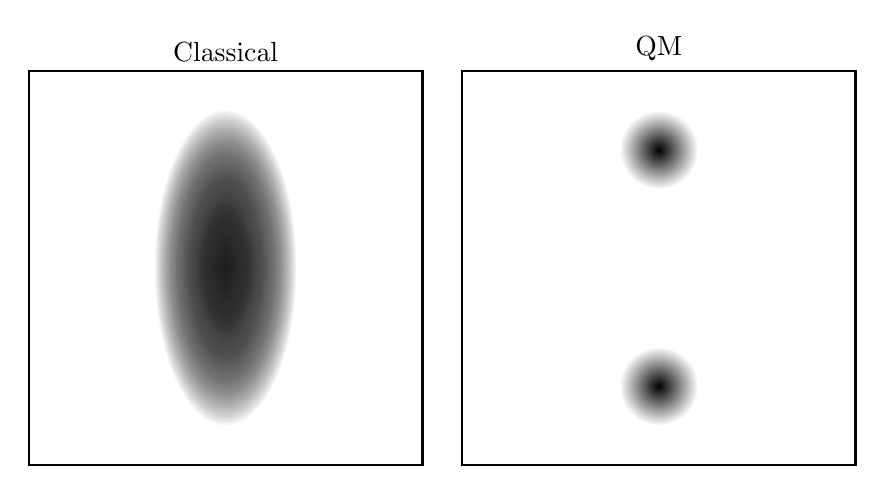
\begin{tikzpicture}[scale=1]
        \shade[even odd rule,inner color=black,outer color=white] (0,0) circle (0.5);
        \shade[even odd rule,inner color=black,outer color=white] (0,-3) circle (0.5);
        \draw[thick] (-2.5, -4) -- (-2.5, 1) -- (2.5, 1) -- (2.5, -4) -- cycle;
        \node[above] at (0, 1) {QM};

        \def\particles{(-5.5,-1.5) }
        \foreach \point in \particles{
        \foreach\i in {0,0.01,...,1.5} {
        \fill[opacity=\i*0.02,black] \point circle ({0.6-\i} and {1-2*\i});         
        }}
        \draw[thick] (-8, -4) -- (-8, 1) -- (-3, 1) -- (-3, -4) -- cycle;
        \node[above] at (-5.5, 1) {Classical};
    \end{tikzpicture}
    \caption{Classical prediction (left) and quantum mechanical prediction (right) for the Stern-Gerlach experiment. The screen on the right was observed in experiment.}
    \label{fig-SGexppredictions}
\end{figure}

How do we interpret this result? We can associate the top dot with spins fully polarized upwards ($\uparrow$) and the bottom dot with spins fully polarized downwards ($\downarrow$). But why is there no signature for sideways pointing spins? We first will answer how a general spin (1/2) state can be represented. If $\ket{\uparrow}$ represents the spin-up state and $\ket{\downarrow}$ represents the spin-down state, then a general spin (and hence sideways spins) can be represented as complex superpositions of these two states, i.e.
\begin{equation}
    \ket{\psi} = \alpha\ket{\uparrow} + \beta\ket{\downarrow}
\end{equation}
where $\alpha, \beta \in  \CC$. What happens in a measurement is then that one element of this general superposition is picked with some probability; indeed, quantum measurement is a probabilistic process. Specifically, we find according to the Born rule that the probability that we measure the spin to be up is $p(\uparrow) = \abs{\uparrow}^2$ and the probability that we measure the spin to be down is $p(\downarrow) = \abs{\downarrow}^2$. Since we require that we measure either spin-up or spin-down, we obtain the normalization condition:
\begin{equation}
    p(\uparrow) + p(\downarrow) = \abs{\alpha}^2 + \abs{\beta}^2 = 1.
\end{equation}
The spin state after the measurement is then $\ket{\uparrow}$ or $\ket{\downarrow}$ respectively, according to the Dirac projection postulate. We will return to these two postulates of quantum mechanics and discuss them in full generality shortly. 

However, we will however make a second comment about measurement before concluding this section. Namely, we consider the case where we perform a repeated measurement of the $z$-component of the spin. As discussed above, the initial general spin state is given by $\ket{\psi} = \alpha\ket{\uparrow} + \beta\ket{\downarrow}$. We then measure the $z$-component of spin and the post-measurement spin state is $\ket{\uparrow}$ or $\ket{\downarrow}$ with probability $\abs{\alpha}^2$ and $\abs{\beta}^2$ respectively. What happens if we measure the $z$-component of spin again? We might think that again, we have probability $\abs{\alpha}^2$ of measuring spin-up and probability $\abs{\beta}^2$ of measuring spin-down. But this is \emph{not} the case. If we measured spin-up in the first measurement, we will measure spin-up in the second measurement with probability one. Similarly, if we measured spin-down in the first measurement, we will measure spin-down in the second measurement with probability one. Evidently, the first measurement has done something to the spin such that the measurement probabilities for the second measurement have been affected (they are not the same as the first). This tells us that quantum measurement is a active process that influences the state of the system we measure. Specifically, it is an irreversible process; there is no notion of ``undo''-ing the measurement to recover the initial (pre-measurement) state.


\subsection{Kets, Bras, and Hilbert Space}
Our goal of the initial stages of this course will be to understand the following table:

\begin{table}[htbp]
    \centering\begin{tabular}{|c|c|}
        \hline Quantum states & $\ket{\psi} \in \H$ 
        \\ \hline Evolution & $i\hbar\pd{}{t}\ket{\psi} = H\ket{\psi}$
        \\ \hline Measurement & $\ket{\psi} \mapsto \frac{\Pi_j \ket{\psi}}{\sqrt{\bra{\psi}\Pi_j\ket{\psi}}} \quad p(j) = \bra{\psi}\Pi_j\ket{\psi}$
        \\ \hline
    \end{tabular}
    \caption{Axioms of quantum mechanics, concerning states, evolution, and measurement.}
    \label{table-QMaxioms}
\end{table}

We will discuss the axioms for quantum states and quantum measurement in this chapter, and the axiom for quantum evolution (which readers may recognize as the Schr\"{o}dinger equation in basis independent form) in the next. It is worth noting that these are the \emph{fundamental postulates} of quantum mechanics; like Newton's laws of motion in classical mechanics, they cannot be derived. We are only able to interpret them, check if they are consistent, and work out the implications.

Let's start the axiom for quantum states; after all it will helpful to know what the objects of our interest are, before we start to work with them! 

\begin{axiombox}{: Quantum states}\label{axiom-states}
    Quantum states $\ket{\psi}$ are vectors (also called ``kets'') in a complex Hilbert space $\H$.
\end{axiombox}

The above axiom is only meaningful if we know what a Hilbert space is; its definition is below:

\begin{defbox}{: (Complex) Hilbert spaces}\label{def-Hilbertspaces}
    $\H$ is a (complex) Hilbert space if:
    \begin{enumerate}[(i)]
        \item $\H$ is a vector space over $\CC$
        \item $\H$ has an inner product
        \item $\H$ is complete (with respect to the metric induced by the norm induced by the inner product)\footnotemark - For the purposes of this course, this last point can be ignored.
    \end{enumerate}
\end{defbox}
\footnotetext{This is a technical qualification for the mathematicians in the crowd. An intuitive explanation for the curious; the inner product on a Hilbert spaces creates a notion of distance on the space. There are sequences (of vectors) that get closer together over time; completeness tells us that any such sequences (known as Cauchy sequences) must converge to a limit.}

Note that the vector space axioms for closure imply that $\forall \ket{\psi}, \ket{\phi} \in \H$ (where $\forall$ means ``for all'') and $\forall c \in \CC$, then $\ket{\psi} + \ket{\phi} \in \H$ and $c\ket{\psi} \in \H$. This tells us that the superposition of quantum states is well defined!

An example which we will return to time and time again (and have already encountered once) is the Hilbert space for a spin-1/2 system. In this case, $\H = \CC^2$. A question that may be brooding in the reader's mind may be ``why do we have to use complex numbers?''; one may indeed wonder if real Hilbert spaces may suffice to do quantum mechanics. The response is negative; we indeed need complex numbers! As an illustrative example, consider again the general spin-1/2 state $\ket{\psi} = \alpha\ket{\uparrow} + \beta\ket{\downarrow}$. Suppose we want a state that has equal probability to be measured spin-up or spin-down under a measurement of the $z$-component of spin. Since $p(\uparrow) = \abs{\alpha}^2$ and $p(\downarrow) = \abs{\beta}^2$, in order to have equal probability we must have $\abs{\alpha} = 1/\sqrt{2}$ and $\abs{\beta} = 1/\sqrt{2}$. A spin pointing in the $+x$ or $-x$ directions indeed has equal weight of up and down. Up to an overall (irrelevant) minus sign, without using complex numbers there are two ways to superimpose $\ket{\uparrow}$ and $\ket{\downarrow}$, from which we can define states corresponding to spins fully polarized in $\pm x$:

\begin{equation}\label{eq-xpm}
    \ket{x, \pm} = \frac{\ket{\uparrow} \pm \ket{\downarrow}}{\sqrt{2}}.
\end{equation}
However, the $\pm \hat{x}$ and $\pm \hat{y}$ vectors lie in the same $z = 0$ plane, and by symmetry we should require that the $\ket{y, \pm}$ would also have equal weights of $\ket{\uparrow}$ and $\ket{\downarrow}$. But if we limit ourselves to real numbers only, we have already exhausted all possible equal-weight combinations of $\ket{\uparrow}$ and $\ket{\downarrow}$ in Eq. \eqref{eq-xpm}. We therefore require complex  numbers to represent all possible states (and indeed, we find that $\ket{y, \pm} = \frac{\ket{\uparrow} \pm i \ket{\downarrow}}{2}$).

Having motivated the ``complex'' in the complex vector space part of the definition of Hilbert spaces, let us now motivate the inner product. We want some way to compare quantum states to one another. Our geometric intuition tells us that the states $\ket{\uparrow}$ and $\ket{\nearrow}$ are ``close'' to each other, while $\ket{\uparrow}$ and $\ket{\downarrow}$ are very ``different''. In order to make this intuition rigorous, we define the inner product, and as a prerequisite we define the dual correspondence.

\begin{defbox}{: Dual correspondence}\label{def-dualcorrespondence}
    To each vector space $\H$, there exists a dual vector space $\H^*$. There is a one-to-one correspondence\footnotemark between the kets $\ket{\psi} \in \H$ and the bras\footnotemark $\bra{\psi} \in \H^*$. We call this the \emph{dual correspondence}, and write it as follows:
    \begin{equation}
        \ket{\psi} \DC \bra{\psi}.
    \end{equation}
    It has the following properties:
    \begin{enumerate}[(i)]
        \item $\ket{\psi} + \ket{\phi} \DC \bra{\psi} + \bra{\phi}$
        \item $c\ket{\psi} \DC c^*\bra{\psi}$
    \end{enumerate}
    where the $*$ denotes complex conjugation.
\end{defbox}
\footnotetext{Formally, this follows from the Riesz Representation Theorem. But for the purposes of this course, we take this one-to-one correspondence as a postulate. Curious readers can find discussions/proofs of the theorem in any text on functional analysis, or mathematical quantum theory.}
\footnotetext{Given such names because $\braket{}{}$ is a bracket - bra-ket. Physicists remain unmatched in their sense of humour.}

Having established the dual correspondence, we may now define the inner product:

\begin{defbox}{: Inner Product}\label{def-innerproduct}
    We define the inner product between $\ket{\psi} \in \H$ and $\ket{\phi} \in \H$ as:
    \begin{equation}
        \braket{\phi}{\psi} \in \CC
    \end{equation}
    with the properties:
    \begin{enumerate}[(i)]
        \item $\braket{\phi}{\psi} = \braket{\psi}{\phi}^*$
        \item $\braket{\psi}{\psi} \geq 0, \forall \ket{\psi} \in \H$
        \item $\braket{\psi}{\psi} = 0 \implies \ket{\psi} = \v{0}$.
    \end{enumerate}
\end{defbox}
Note that $\v{0}$ in the above definition is the null ket (also known as the zero vector, which must be an element of the Hilbert space), where $\v{0} = 0\ket{\psi}, \forall \ket{\psi}$. It is an unphysical state. We normally work with normalized states, i.e. states $\ket{\psi}$ that satisfy $\braket{\psi}{\psi} = 1$. The null ket has inner product zero and cannot be normalized.

As a first use of the inner product, let us return to our initial motivation for obtaining the ``likeness'' of states. For normalized states, it follows (and we will later prove) that:
\begin{equation}
    0 \leq \abs{\braket{\phi}{\psi}} \leq 1.
\end{equation}
We therefore can use the inner product as a method to evaluate the likeness of states. $\braket{\phi}{\psi} = 0$ means that $\ket{\psi}$ and $\ket{\phi}$ are maximally different, and $\abs{\braket{\phi}{\psi}} = 1$ corresponds to $\ket{\psi}$ and $\ket{\phi}$ being the same.

\newpage
\section[Quantum Dynamics]{\hyperlink{toc}{Quantum Dynamics}}

\subsection{Introduction to the Schr\"{o}dinger Equation}
Recall Table \ref{table-QMaxioms} which laid out the axioms of quantum mechanics; up until this point we have discussed quantum states, as well as quantum measurement (projective dynamics) - we will now discuss the last entry in the table, which concerns the unitary dynamics/evolution of quantum states.

\begin{axiombox}{: The Schr\"{o}dinger Equation}\label{axiom-SE}
    The evolution of a quantum state $\ket{\psi(t)}$ evolving under the influence of a Hamiltonian operator $H$ (which describes the energy of the system) is given by the Schr\"{o}dinger Equation:
    \begin{equation}\label{eq-SEbasisindep}
        i\hbar\dpd{}{t}\ket{\psi(t)} = H\ket{\psi(t)}
    \end{equation}
\end{axiombox}

Many quantum phenomena can be derived from the Schr\"{o}dinger equation; for example the shape of orbitals and the energy spectra of the Hydrogen atom, which is a system you (hopefully) solved in a previous course.

\begin{figure}[htbp]
    \centering
    \includegraphics[scale=0.1]{Images/HHespectrum.png}
    \caption{Emission spectrum of Hydrogen and Helium, which can be derived by analyzing the Schr\"{o}dinger equation (though we note that the Hydrogen atom is one of the (very few) systems which are analytically solvable, and the Helium atom must be treated by approximation techniques). Image created by Ranjithsiji, licensed under the \href{https://creativecommons.org/licenses/by-sa/4.0/deed.en}{Creative Commons Attribution-Share Alike 4.0 International license}. }
    \label{fig-HHespectrum}
\end{figure}

Above, we give the basis-independent form of the Schr\"{o}dinger equation. This differs from the form of the SE that you might be more familiar with, which likely takes the form as in Eq. \eqref{eq-SEintro}. This form is the SE written in the position basis; we will begin by deriving this form (in 1-D) from the general/basis-independent equation.

In general, the energy (Hamiltonian) operator $H$ has two terms, a (position-dependent) potential term and a kinetic term:
\begin{equation}\label{eq-generalH}
    H = \underbrace{V(X)}_{\text{potential}} + \underbrace{\frac{P^2}{2m}}_{\text{kinetic}}
\end{equation}
where $X, P$ are the position/momentum operators and $m$ is the mass of the particle. Some familiar forms of $V$ you may have encountered in previous courses are $V(X) = 0$ for the free particle, $V(X) = \frac{1}{2}m\omega^2X^2$ for the quantum harmonic oscillator (which we will discuss later in this chapter), and $V(R) = -\frac{e^2}{4\pi \e_0}\frac{1}{R}$ for the Hydrogen atom.

Let us now express this basis-independent expression of the Hamiltonian in the position basis. 

\begin{propbox}{: Schr\"{o}dinger equation in position basis}
    In the position basis, the Schr\"{o}dinger equation with Hamiltonian Eq. \eqref{eq-generalH} reads:
    \begin{equation}\label{eq-SEpositionbasis}
        i\hbar\dpd{}{t}\psi(x, t) = \left[V(x, t) -\frac{\hbar^2}{2m}\dpd[2]{}{x}\right]\psi(x, t)
    \end{equation}
\end{propbox}

\begin{proof}
    Starting with the potential term, we have:
    \begin{equation}
        \begin{split}
            V(X) &= \left(\int dx \dyad{x}{x}\right)V(X)\left(\int dx' \dyad{x'}{x'}\right)
            \\ &= \int dxdx' \ket{x}\left(\bra{x}V(X)\ket{x'}\right)\bra{x'}
            \\ &= \int dxdx' \ket{x}V(x')\braket{x}{x'}\ket{x'}
            \\ &= \int dxdx' \ket{x} V(x')\delta(x-x')\ket{x'}
            \\ &= \int dx \ket{x}V(x)\bra{x}
        \end{split}
    \end{equation}
    where we have inserted the resolution of the identity twice in the first line, used that $V(X)\ket{x'} = V(x')\ket{x'}$ (eigenvalue equation for position) in the third line, and used the orthonormality of the position basis in the fourth line.

    For the kinetic term, we have:
    \begin{equation}
        \begin{split}
            P^2\ket{\psi} &= \left(\int dx \dyad{x}{x}\right) P \left(\int dx' \dyad{x'}{x'}\right) P\ket{\psi}
            \\ &= \int dxdx' \ket{x}\left(\bra{x}P\ket{x'}\right)\left(\bra{x'}P\ket{\psi}\right)
            \\ &= (-i\hbar)^2 \int dxdx' \ket{x} \dpd{}{x}\braket{x}{x'} \dpd{}{x'}\dpd{x'}{\psi}
            \\ &= -\hbar^2 \int dxdx' \ket{x}\dpd{}{x}\delta(x-x')\dpd{}{x'}\braket{x'}{\psi}
            \\ &= -\hbar^2 \int dx \ket{x} \dpd{}{x}\dpd{}{x}\braket{x}{\psi}
            \\ &= -\hbar^2 \int dx\ket{x} \dpd[2]{}{x}\braket{x}{\psi}
        \end{split}
    \end{equation}
    Where in the first equality we insert the resolution of the identity twice, in the third equality we used the previously derived expression for momentum in the position basis (Eq. \eqref{eq-momentumXbasis}), in the fourth equality we use the orthonormality of the position basis, and we use the subsequent dirac delta to carry out the integrals. Now if we multiply by a position eigenbra on both sides, we have:
    \begin{equation}
        \begin{split}
            \bra{x}P^2\ket{\psi} &= \bra{x}\left(-\hbar^2 \int dx'\ket{x'} \dpd[2]{}{x'}\braket{x'}{\psi}\right)
            \\ &= -\hbar^2 \int dx' \braket{x}{x'}\dpd[2]{}{x'}\braket{x'}{\psi}
            \\ &= -\hbar^2 \int dx' \delta(x - x')\dpd[2]{}{x'}\braket{x'}{\psi}
            \\ &= -\hbar^2 \dpd[2]{}{x}\braket{x}{\psi}
        \end{split}
    \end{equation} 
    We conclude that:
    \begin{equation}
        \bra{x}P^2\ket{\psi} = -\hbar\dpd[2]{}{x} \braket{x}{\psi}
    \end{equation}
    Putting it all together; let us multiply the basis-independent SE (Eq. \eqref{eq-SEbasisindep}) on the right by a position eigenbra:
    \begin{equation}
        \bra{x}i\hbar\dpd{}{t}\ket{\psi} = \bra{x}H\ket{\psi} = \bra{x}V(x)\ket{\psi} + \bra{x}\frac{P^2}{2m}\ket{\psi}
    \end{equation}
    The prior results then yield:
    \begin{equation}
        i\hbar\dpd{}{t}\braket{x}{\psi} = V(x)\braket{x}{\psi} - \frac{\hbar^2}{2m}\dpd[2]{}{x}\braket{x}{\psi}
    \end{equation}
    and since $\braket{x}{\psi}$ is just the position wavefunction, we have now successfully derived the (familiar) 1-D SE in the position basis (also, let us now insert the time parameter into the wavefunction and the potential, as the wavefunction is time-dependent and the potential also can be time-dependent depending on the system; e.g. a time-varying magnetic field):
    \begin{equation}
        i\hbar\dpd{}{t}\psi(x, t) = \left[V(x, t) -\frac{\hbar^2}{2m}\dpd[2]{}{x}\right]\psi(x, t)
    \end{equation}
\end{proof}
In 3D we have the generalization:
\begin{equation}
    i\hbar\dpd{}{t}\psi(\v{r}, t) = \left[V(\v{r}, t) - \frac{\hbar^2}{2m}\nabla^2\right]\psi(\v{r}, t)
\end{equation}
where:
\begin{equation}
    \nabla^2 = \dpd[2]{}{x} + \dpd[2]{}{y} + \dpd[2]{}{z}
\end{equation}
is the Laplacian.

\subsection{Spin Precession and Medical Imaging}
Let us explore a concrete example of Schr\"{o}dinger evolution of a quantum system. Namely, we analyze how a spin-1/2 system evolves in a constant magnetic field.

Classically, the energy of a magnetic dipole with dipole moment $\v{m}$ in a magnetic field $\v{B}$ is given by:
\begin{equation}
    E = -\v{m} \cdot \v{B}
\end{equation}
with the minus sign present as it is energetically favourable for the dipole to align with the magnetic field. In analogy, the quantum mechanical Hamiltonian for the system is given by:
\begin{equation}
    H = -\frac{e}{m_e c}\v{S} \cdot \v{B}
\end{equation}
with $e$ the charge of the electron, $m_e$ the mass of the electron, $c$ the speed of light, and $\v{S} = (S_x, S_y, S_z)^T$ a vector of spin operators. Let us suppose that we have a constant field aligned in the $\zhat$ direction, so $\v{B} = B\zhat$. Then the above reduces to:
\begin{equation}
    H = -\frac{eB}{m_e c}S_z
\end{equation}
Defining $\omega = \frac{\abs{e}B}{m_e c}$, and recalling that the electron charge is negative, the Hamiltonian can be written as:
\begin{equation}
    H = \omega S_z
\end{equation}
The choice of notation $\omega$, traditionally used to represent some frequency, will become clear shortly.

We now look at how an electron spin, originally prepared in the spin state $\ket{\psi(0)} = \ket{+} = \frac{\ket{\uparrow} + \ket{\downarrow}}{\sqrt{2}}$, evolves under the influence of this Hamiltonian; that is, we wish to solve the time-dependent SE:
\begin{equation}\label{eq-spinprecessSE}
    i\hbar\dpd{}{t}\ket{\psi(t)} = \omega S_z\ket{\psi(t)}
\end{equation}

First, we recall the eigenstates and eigenvalues of $S_z$, namely that $S_z\ket{\uparrow/\downarrow} = \pm \frac{\hbar}{2}\ket{\uparrow/\downarrow}$ and hence taking the dual $\bra{\uparrow/\downarrow}S_z = \pm \bra{\uparrow/\downarrow}\frac{\hbar}{2}$. Now, multiplying Eq. \eqref{eq-spinprecessSE} on the right with $\bra{\uparrow}$, we find:
\begin{equation}
    \bra{\uparrow}i\hbar\dpd{}{t}\ket{\psi(t)} = \bra{\uparrow}\omega S_z \ket{\psi(t)} \implies i\hbar\dpd{}{t}\braket{\uparrow}{\psi(t)} = \omega\bra{\uparrow}\frac{\hbar}{2}\ket{\psi(t)} \implies i\hbar\dpd{}{t}\psi_\uparrow(t) = \frac{\hbar\omega}{2}\psi_\uparrow(t)
\end{equation}
where $\psi_\uparrow(t) \coloneqq \braket{\uparrow}{\psi(t)}$ (the ``spin-up'' component of $\ket{\psi(t)}$). Analogously we find:
\begin{equation}
    i\hbar\dpd{}{t} = -\frac{\hbar\omega}{2}\psi_\downarrow(t)
\end{equation}
In matrix form we can express this system of two ODEs (making the identification $\ket{\uparrow} \cong (1, 0)^T, \ket{\downarrow} \cong (0, 1)^T$) as:
\begin{equation}
    i\hbar\dpd{}{t}\m{\psi_\uparrow(t) \\ \psi_\downarrow(t)} = \frac{\hbar\omega}{2}\m{1 & 0 \\ 0 & -1}\m{\psi_\uparrow(t) \\ \psi_\downarrow(t)}
\end{equation}
These equations are easily solved by inspection to be complex exponentials (you can check!):
\begin{equation}
    \psi_\uparrow(t) = c_\uparrow e^{-\frac{i\omega}{2}t}, \quad \psi_\downarrow(t) = c_\downarrow e^{\frac{i\omega}{2} t}
\end{equation}
Where the coefficients $c_\uparrow, c_\downarrow$ are determined by the initial state $\ket{\psi(0)}$:
\begin{equation}
    c_\uparrow = \braket{\uparrow}{\psi(0)} = \frac{1}{\sqrt{2}}
\end{equation}
\begin{equation}
    c_\downarrow = \braket{\downarrow}{\psi(0)} = \frac{1}{\sqrt{2}}
\end{equation}
From which we conclude the solution to the SE in this case to be:
\begin{equation}\label{eq-spinprecesssoln}
    \ket{\psi(t)} = \frac{1}{\sqrt{2}}e^{-\frac{i\omega}{2}t}\ket{\uparrow} + \frac{1}{\sqrt{2}}e^{\frac{i\omega}{2} t}\ket{\downarrow}.
\end{equation}

Two comments before we move on; eigenstates of Hamiltonians do not evolve in time (except for a physically irrelevant phase factor $e^{-i\frac{E_n}{\hbar}t}$) - so if we instead started with state $\ket{\psi(0)} = \ket{\uparrow}$, the spin would be fully polarized upwards for all time and would not be influenced by the ($\zhat$-oriented) external magnetic field. Yet again, we see that it is the relative phase that has physically observable effects.

On this note of eigenstates of a Hamiltonian begin stationary in time (hence sometimes called ``stationary states''), we have the following generic recipe for solving the SE (in the case where we have a time-independent Hamiltonian $H$):
\begin{enumerate}
    \item Solve for the eigenenergies $E_n$ and corresponding eigenvectors $\ket{n}$ of $H$ (Note - while this is generally fairly simple for small finite-dimensional systems, this is exceptionally difficult when we consider the continuous case (there are exceptionally few potentials that can be analytically solved), or systems with an infinite number of spins - for these we require approximation techniques, which we will discuss towards the end of the course). The evolution of these stationary states is just via the complex phase factor, e.g. $e^{-i\frac{E_n}{\hbar}t}\ket{n}$. 
    \item Expand out the initial state $\ket{\psi(0)}$ in the eigenbasis of $H$, i.e. $\ket{\psi(0)} = \sum_n \braket{n}{\psi(0)}\ket{n}$ via resolution of the identity.
    \item Solve for $\ket{\psi(t)}$ by considering the evolutions of each of the eigenstates independently, and then by linearity:
    \begin{equation}
        \ket{\psi(t)} = \sum_n \braket{n}{\psi(0)} e^{-i\frac{E_n}{\hbar}t}\ket{n}.
    \end{equation}
\end{enumerate}

Now, let's return back to our current example of the spin-1/2 particle in a magnetic field. Let's calculate the expectation value of $S_x$ as a function of time:
\begin{equation}
    \begin{split}
        \avg{S_x}_\psi(t) &= \bra{\psi(t)}S_x\ket{\psi(t)}
        \\ &= \left(\frac{1}{\sqrt{2}}e^{\frac{i\omega}{2}t}\bra{\uparrow} + \frac{1}{\sqrt{2}}e^{-\frac{i\omega}{2} t}\bra{\downarrow}\right)S_x\left(\frac{1}{\sqrt{2}}e^{-\frac{i\omega}{2}t}\ket{\uparrow} + \frac{1}{\sqrt{2}}e^{\frac{i\omega}{2} t}\ket{\downarrow}\right)
        \\ &= \left(\frac{1}{\sqrt{2}}e^{\frac{i\omega}{2}t}\bra{\uparrow} + \frac{1}{\sqrt{2}}e^{-\frac{i\omega}{2} t}\bra{\downarrow}\right)\frac{\hbar}{2}\left(\frac{1}{\sqrt{2}}e^{-\frac{i\omega}{2}t}\ket{\downarrow} + \frac{1}{\sqrt{2}}e^{\frac{i\omega}{2} t}\ket{\uparrow}\right)
        \\ &= \frac{\hbar}{4}\left(\braket{\uparrow}{\downarrow} + e^{i\omega t}\braket{\uparrow}{\uparrow} + e^{-i\omega t}\braket{\downarrow}{\downarrow} + \braket{\downarrow}{\uparrow}\right)
        \\ &= \frac{\hbar}{4}\left(e^{i\omega t} + e^{-i\omega t}\right)
        \\ &= \frac{\hbar}{2}\cos(\omega t)
    \end{split}
\end{equation}
where we have used that $S_x\ket{\uparrow/\downarrow} = \frac{\hbar}{2}\ket{\downarrow/\uparrow}$, the orthonormality of the up/down spin states and an Euler identity of $\frac{e^{i\omega t} + e^{-i\omega t}}{2} = \cos(\omega t)$. We see that the expectation value of $S_x$ precesses in time! Note that the expectation value of $S_y$ similarly precesses, with an analogous calculation showing that $\avg{S_y}_{\psi(t)} = \frac{\hbar}{2}\sin(\omega t)$. $S_z$ commutes with the Hamiltonian and hence its expectation value is constant in time; and since $\bra{\psi(0)}S_z\ket{\psi(0)} = \bra{+}S_z\ket{+} = \frac{\hbar}{2}\braket{+}{-} = 0$, $\avg{S_z}_{\psi(t)} = 0$ for all time.

We can visualize this precession of the spin using the \emph{Bloch sphere} representation of a spin-1/2 (qubit) system. The state $\ket{\psi(t)}$ that we solved for in Eq. \eqref{eq-spinprecesssoln} can be visualized as a vector rotating along the surface of the unit sphere in the $xy$-plane:

\begin{figure}[htbp]
    \centering
    \includegraphics{Images/fig-spinprecess.pdf}
    \caption{Bloch sphere visualization of spin precession; $\ket{\psi(t)}$ precesses in the $xy$-plane with frequency $\omega$.}
    \label{fig-spinprecess}
\end{figure}


We will return to this Bloch sphere representation when we begin our discussion of quantum information; nevertheless, you might find the following exercise interesting; consider the spin operator in the $\hat{\v{n}}$ direction, given by $S_{\hat{\v{n}}} = \v{S} \cdot \hat{\v{n}}$. Parameterizing in polar coordinates, we can write $\hat{\v{n}} = (n_x, n_y, n_z)^T = (\sin\theta\cos\phi, \sin\theta\sin\phi, \cos\theta)^T$. You can check that the ($+\hbar/2$) eigenvector for this operator can be solved to be:
\begin{equation}\label{eq-nhatspin}
    \ket{+\hat{\v{n}}} = \cos(\frac{\theta}{2})\ket{\uparrow} + e^{i\phi}\sin(\frac{\theta}{2})\ket{\downarrow}
\end{equation}
in the Bloch sphere representation, this can be realized as the vector with polar angle $\theta$ and azimuthal angle $\phi$.

\begin{figure}[htbp]
    \centering
    \includegraphics{Images/fig-Blochsphere.pdf}
    \caption{Bloch sphere representation of the spin-1/2 state $\ket{+\hat{\v{n}}} = \cos(\frac{\theta}{2})\ket{\uparrow} + e^{i\phi}\sin(\frac{\theta}{2})\ket{\downarrow}$, which lies on the surface of the unit two-sphere and has polar angle $\theta$ and azimuthal angle $\phi$.}
    \label{fig-Blochsphere}
\end{figure}

Note that Eq. \eqref{eq-nhatspin} is a totally generic spin-1/2 state; naively, one needs two complex numbers, and hence four real parameters to specify the state of a spin-1/2 particle $\ket{\psi} = \alpha\ket{\uparrow} + \beta\ket{\downarrow}$. However, the normalization condition of $\abs{\alpha}^2 + \abs{\beta}^2 = 1$ and the irrelevancy of the global phase of $\ket{\psi}$ means that it is (physically) uniquely specified by two real numbers. 


This example of spin precession is not only of pedagogical interest (being an example of where we can analytically solve the SE, and for arguably the simplest quantum system) but is also of practical interest - namely for medical imaging (i.e.  NMR/MRI). When a (nuclear) spin precesses (under the influence of a $\v{B}$-field; which is why MRI requires such strong magnets) they emit electromagnetic radiation. This can then be picked up by an antenna, where the strength of the electromagnetic signal corresponds to the number of spins precessing, and therefore provides a measurement of the number of spins in a particular sample (e.g. of the brain).

We give an extremely high-level explanation here, as we have not yet developed all the tools necessary to discuss this in all the detail. We consider some sample of spins, where we want to measure the (spatially dependent) spin density. How would we go about doing this?

We begin with a static (time-independent) $\v{B}$-field, which we can WLOG take to be (as we have) in the $\zhat$ direction, so $\v{B} = B\zhat$. Then the energy/Hamiltonian is given by:
\begin{equation}
    E = -\frac{\abs{e}B}{m_p c}S_z
\end{equation}
From the above expression we can see that it is energetically favourable for the spins to align with the static $\v{B}$-field. Specifically, with $\omega = \frac{\abs{e}B}{m_p c}$, we have that the spin-up states have eigenenergy $-\frac{\hbar\omega}{2}$, and the spin-down states have eigenenergy $\frac{\hbar\omega}{2}$. The two states have energy difference $\Delta E = \hbar \omega$.

The stronger this static magnetic field is, the more spins in our sample will be aligned with it (there will be some anti-aligned population, due to thermal excitations; the strength of the magnetic field then determines how much more likely the spins are to be in the ground (aligned) state, with the excited (anti-aligned) spins supressed by a Boltzmann factor $e^{-\hbar \omega/k T}$), and hence the stronger the net magnetization of the spins. However, this static field alone cannot yield a precession signal, as the aggregate spin vector does not precess here; it is just aligned with the $\v{B}$-field. The individual spins may exhibit some precession about $\zhat$ (as the quantum mechanical picture is that each spin in the sample is some superposition of the up/down spin states, and therefore can precess) but the phase of a given spin is random, and so when adding up to form the aggregate spin vector we find $\avg{S_x} = \avg{S_y} = 0$ and no precession is observed. 

What we require then to obtain a precession signal is a second external magnetic field. Specifically, a field that is time-dependent, and rotating in the $xy$-direction with time:
\begin{equation}
    \v{B}(t) = B_1(\xhat\cos(\omega' t) + \yhat\sin(\omega' t))
\end{equation}
This time-dependent rotating field (which we do not know how to analyze yet - stay tuned for the treatment of time-dependent Hamiltonians and the Rabi formula, to come at the end of this course!) causes $p_\uparrow(t)$ and $p_\downarrow(t)$ to be time dependent (unlike the static $\v{B} = B\zhat$ field, which cannot cause changes in the up/down components of the spins in time); that is, we see spin ``flips'' in addition to spin precession from just the static magnetic field. Specifically, the probability of such spin flips is maximized when the rotating magnetic field frequency $\omega'$ matches the precession frequency $\omega$, i.e. we have the resonance condition $\omega' = \omega$. You can picture this rotating magnetic field (when pulsed for an appropriate amount of time) as having the effect of ``tipping'' the aggregate magnetization vector into the $xy$-plane, and such the aggregate spin can precess and we are able to read out a (strong) EM signal from our sample.

\begin{figure}[htbp]
    \centering
    \includegraphics{Images/fig-Rabi.pdf}

    \caption{A RF (radiofrequency) field (rotating magnetic field) at the resonance frequency of $\omega' = \omega$ maximizes the probability of ``spin flips'' between the ground ($\uparrow$/ aligned) state to the excited ($\downarrow$/anti-aligned) state.}
    \label{fig-Rabi}
\end{figure}

\begin{figure}[htbp]
    \centering
    \includegraphics{Images/fig-spintipping.pdf}

    \caption{Applying a pulse of the (time-dependent) RF field causes the upwards-polarized (and therefore non-precessing) aggregate spin vector to tip into the $xy$-plane, where a maximal amount of precession signal can be read out.}
    \label{fig-spintipping}
\end{figure}

How do we now introduce spatial resolution into this picture? Since the resonance frequency $\omega$ is dependent on the static field strength $B$, an approach is then to make the static $B$ field position dependent; this changes the resonance condition depending on where in the sample we are. This is illustrated in Fig. \ref{fig-1DBgradient} below, where we have the static field strength varying in one dimension.

\begin{figure}[htbp]
    \centering
    \includegraphics{Images/fig-1DBgradient.pdf}

    \caption{By applying a $B$-field with a gradient (here, increasing linearly as we go to the right) along the sample, the resonance frequency changes proportional to the $B$-field strength.}
    \label{fig-1DBgradient}
\end{figure}

In three dimensions (of prime interest for imaging) we can use spatially dependent fields to get a signal from a specifically chosen 2D plane only. We can then vary this plane to get spatial resolution.

Let us go through an example in 2D; suppose we have a sample with spin-polarizable matter in the center. We can then consider varying the magnetic field over two planes, namely going vertically and horizontally through the sample. Based on the precession signal we extract (peaking at $x = y = 0$) we are able to resolve the sample.

\begin{figure}[htbp]
    \centering
    \includegraphics{Images/fig-2DBgradient.pdf}
    
    \caption{Simple example of 2D medical imaging. Suppose we have a sample with spin-polarizable matter in the center. By applying a vertical and horizontal gradient across the sample and measuring the signal strength, we are able to localize the spin-polarizable matter within the sample.}
    \label{fig-2DBgradient}
\end{figure}

For general density patterns in 3D, we can choose multiple planes that go through the sample (over which we vary the $B$-field strength) in order to resolve it.

\subsection{Unitarity of Schr\"{o}dinger Evolution}

We make an observation about our previous example of spin precession; we found that for intitial state $\ket{\psi(0)} = \ket{+}$ the state through time would be:
\begin{equation}
    \ket{\psi(t)} = \frac{1}{\sqrt{2}}e^{-\frac{i\omega}{2}t}\ket{\uparrow} + \frac{1}{\sqrt{2}}e^{\frac{i\omega}{2}t}\ket{\downarrow}.
\end{equation}
and if we started with state $\ket{\phi(0)} = \ket{\uparrow}$ the state through time would be:
\begin{equation}
    \ket{\phi(t)} = e^{-\frac{i\omega}{2}t}\ket{\uparrow}
\end{equation}
and so we notice that:
\begin{equation}
    \braket{\phi(t)}{\psi(t)} = \left(e^{\frac{i\omega}{2}t}\bra{\uparrow}\right)\left(\frac{1}{\sqrt{2}}e^{-\frac{i\omega}{2}t}\ket{\uparrow} + \frac{1}{\sqrt{2}}e^{\frac{i\omega}{2}t}\ket{\downarrow}\right) = \frac{1}{\sqrt{2}}\braket{\uparrow}{\uparrow} + \frac{1}{\sqrt{2}}e^{i\omega t}\braket{\uparrow}{\downarrow} = \frac{1}{\sqrt{2}}
\end{equation}
for all times $t$! That is, angles seem to be preserved under Schr\"{o}dinger evolution. We can also visualize this angle preservation in the Bloch sphere representation; looking at Fig. \ref{fig-spinprecess}, you can see that the angle (of $\theta = \pi/2$) between the $\ket{\uparrow}$ state (aligned along $\zhat$) and the precessing spin in the $xy$-plane stays constant in time, even as the spin evolves.


Now, is this property generally true, or is this just a special case? It turns out that yes, it always holds for \emph{any} two states $\ket{\psi}, \ket{\phi}$ (which belong to an arbitrary Hilbert space) that Schr\"{o}dinger evolution preserves the inner product:
\begin{equation}
    \braket{\phi(t)}{\psi(t)} = \braket{\phi(0)}{\psi(0)}.
\end{equation}

This statement is actually quite striking, given our experience in classical mechanics; given a classical ODE, two solutions can diverge in time (for example: consider the trajectory of an object thrown at two different initial velocities; even though the objects may start at the same position, the distance between them will grow apart in time). However, in QM the ``distance'' between states is fixed in time! A potential question that may arise: how do we explain chaos? Chaotic systems (that is, systems highly sensitive to initial conditions, where very slight differences can lead to vastly different future behaviour) are everywhere, for example the weather and $N$-body systems. Yet if quantum mechanics is the more correct theory underlying physics (where such diverging behaviour simply does not occur under evolution by the Schr\"{o}dinger equation, as we will now prove), where does such chaotic behaviour arise?

We leave the reader to ponder the above question, and move onto the proof that Schr\"{o}dinger evolution is unitary; from this the inner product preserving property will follow.

\begin{thmbox}{: Unitarity of Schr\"{o}dinger evolution}\label{thm-SEunitary}
    Evolution under the Schr\"{o}dinger equation is unitary. That is, given the time-evolution of a quantum state as goverened by the Schr\"{o}dinger equation:
    \begin{equation}
        i\hbar\dpd{}{t}\ket{\psi(t)} = H\ket{\psi(t)}
    \end{equation}
    we can write $\ket{\psi(t)} = U(t)\ket{\psi(0)}$ where $U(t)$ is the ``time-evolution'' operator. This time evolution operator is unitary.
\end{thmbox}
\begin{proof}
    First, note that writing $\ket{\psi(t)} = U(t)\ket{\psi(0)}$, we can substitute this into the Schr\"{o}dinger equation to obtain:
    \begin{equation}
        i\hbar\dpd{}{t}\left(U(t)\ket{\psi(0)}\right) = H(t)U(t)\ket{\psi(0)}
    \end{equation}
    where we note that in general, the Hamiltonian may have time dependence. Since the above holds for arbitrary initial states $\ket{\psi(0)}$, it follows that:
    \begin{equation}\label{eq-Ut}
        i\hbar\dpd{}{t}U(t) = H(t)U(t)
    \end{equation}
    We now break up our analysis into cases.
    \begin{enumerate}
        \item $\boxed{H \text{ is constant in time}}$. In this case, Eq. \eqref{eq-Ut} is easily solved by inspection:
        \begin{equation}\label{eq-UtHtimeindep}
            U(t) = e^{-i\frac{H}{\hbar}t}
        \end{equation}
        But then taking the Hermitian conjugate, we have:
        \begin{equation}
            U^\dag(t) = e^{i\frac{H^\dag}{\hbar}t} = e^{i\frac{H}{\hbar}t}
        \end{equation}
        as $H$ is Hermitian. Therefore:
        \begin{equation}
            U(t)U^\dag(t) = U^\dag(t) U(t) = \II
        \end{equation}
        and so $U$ is unitary as claimed.

        \item $\boxed{H \text{ depends on time}}$. For this case, note that (by rearranging Eq. \eqref{eq-Ut}) that:
        \begin{equation}\label{eq-dpdUt}
            \dpd{}{t}U(t) = \frac{H(t)}{i\hbar}U(t)
        \end{equation}
        and taking the Hermitian conjugate of the above equation:
        \begin{equation}\label{eq-dpdUdagt}
            \dpd{}{t}U^\dag(t) = -\frac{U^\dag(t)}{i\hbar}H(t)
        \end{equation}
        where we use that $(AB)^\dag = B^\dag A^\dag$ and that $H$ is Hermitian. Now using the product rule:
        \begin{equation}
            \begin{split}
                \dpd{}{t}\left(U^\dag(t) U(t)\right) &= \left(\dpd{}{t}U^\dag(t)\right)U(t) + U^\dag(t)\left(\dpd{}{t}U(t)\right) 
                \\ &= -\frac{1}{i\hbar}U^\dag(t)H(t)U(t) + \frac{1}{i\hbar}U^\dag(t)H(t)U(t)
                \\ &= 0
            \end{split}
        \end{equation}
        It therefore follows that $U^\dag(t)U(t)$ is constant in time, and so $U^\dag(t)U(t) = U^\dag(0)U(0) = \II$ (as at time $t = 0$, the evolution operator does nothing!). The claim is therefore proven. 
    \end{enumerate}
\end{proof}

\begin{corbox}{: Schr\"{o}dinger evolution preserves the inner product}
    For any two quantum states $\ket{\psi(t)}, \ket{\phi(t)}$ evolving under the Schr\"{o}dinger equation:
    \begin{equation}
        \braket{\phi(t)}{\psi(t)} = \braket{\phi(0)}{\psi(0)}
    \end{equation}
\end{corbox}

\begin{proof}
    Writing $\ket{\psi(t)} = U(t)\ket{\psi(0)}$ and $\ket{\phi(t)} = U(t)\ket{\phi(0)}$, we have:
    \begin{equation}
        \braket{\phi(t)}{\psi(t)} = \bra{\phi(0)}U^\dag(t) U(t)\ket{\psi(0)} = \bra{\phi(0)}\II\ket{\psi(0)} = \braket{\phi(0)}{\psi(0)}
    \end{equation}
    where we have used unitarity in the second equality. 
\end{proof}

\subsection{The Heisenberg Picture and Ehrenfest's Theorem}
So far, we have taken the view that quantum states $\ket{\psi}$ are the objects that evolve in time, and that observables are fixed through time. However, this is not the only way to do quantum mechanics. Often, we are interested in the expectation value of an observable $A$ and how this evolves through time -  Does it then make sense to consider observables as the objects that evolve through time, and the states as the fixed objects?

The answer turns out to be yes, and this is what is known as the Heisenberg picture. To see how things work in this picture, let's consider the expectation value of some observable $A$:
\begin{equation}
    \begin{split}
        \avg{A(t)}_\psi &= \bra{\psi(t)}A\ket{\psi(t)}
        \\ &= \left(\bra{\psi(0)}U^\dag(t)\right)A\left(U(t)\ket{\psi(0)}\right)
        \\ &= \bra{\psi(0)}\left(U^\dag(t)A U(t)\right)\ket{\psi(0)}
    \end{split}
\end{equation}
We now define the observable $A$ in the Heisenberg picture to be:
\begin{equation}
    A^H(t) \coloneqq U^\dag(t)A U(t)
\end{equation}
where $A$ is the observable in the (familiar) Schr\"{o}dinger picture, and $U(t)$ is the unitary time-evolution operator. And so, in the Heisenberg picture, the observable is what evolves through time!

If states evolve via the Schr\"{o}dinger equation, what evolution equation does $A^H(t)$ satisfy? Let us now derive it.

\begin{thmbox}{: Heisenberg equation of motion}
    In the Heisenberg picture, the evolution of observables $A^H(t) \coloneqq U^\dag(t) A U(t)$ are governed by the Heisenberg equation of motion:
    \begin{equation}\label{eq-Heisenberggeneral}
        \dod{}{t} A^H(t) = \frac{1}{i\hbar}[A^H(t), H^H(t)]
    \end{equation}
    where $H(t)$ is the Hamiltonian under which the system evolves (and $H^H = U^\dag(t) H(t) U(t)$ its counterpart in the Heisenberg picture). In the case where $H$ is independent of time (which is true for many cases of interest), $H^H(t) = H$ (i.e. the Hamiltonian is the same in the Schr\"{o}dinger and Heisenberg pictures) and so the above simplifies to:
    \begin{equation}\label{eq-Heisenberg}
        \dod{}{t} A^H(t) = \frac{1}{i\hbar}[A^H(t), H]
    \end{equation}
\end{thmbox}
\begin{proof}
    Using the definition of Heisenberg picture operators and the product rule, we have:
    \begin{equation}
        \begin{split}
            \dod{}{t}A^H(t) &= \dod{}{t}\left(U^\dag(t) A U(t)\right)
            \\ &= \left(\dod{}{t}U^\dag(t)\right)A U(t) + U^\dag(t) A \left(\dod{}{t}U(t)\right)
        \end{split}
    \end{equation}
    where we note that the derivative of the Schr\"{o}dinger picture operators is zero since they are independent of time. Now, using Eqs. \eqref{eq-dpdUt}, \eqref{eq-dpdUdagt} (derived from the Schr\"{o}dinger equation) we find:
    \begin{equation}
        \dod{}{t}A^H(t) = -\frac{1}{i\hbar}U^\dag(t) H(t) A U(t) + \frac{1}{i\hbar}U^\dag(t) A H(t) U(t)
    \end{equation}
    Inserting $\II = U(t)U^\dag(t)$ in between the $A$ and $H$s:
    \begin{equation}
        \begin{split}
            \dod{}{t}A^H(t) &= -\frac{1}{i\hbar}U^\dag(t) H(t) U(t)U^\dag(t) A U(t) + \frac{1}{i\hbar}U^\dag(t) A U(t)U^\dag(t) H(t) U(t)
            \\ &= -\frac{1}{i\hbar}\left(U^\dag(t) H(t) U(t)\right)\left(U^\dag(t) A U(t)\right) + \frac{1}{i\hbar}\left(U^\dag(t) A U(t)\right)\left(U^\dag(t) H(t) U(t)\right)
            \\ &= -\frac{1}{i\hbar} H^H(t)A^H(t) + \frac{1}{i\hbar}A^H(t) H^H(t)
            \\ &= \frac{1}{i\hbar}[A^H(t), H^H(t)]
        \end{split}
    \end{equation}
    and so Eq. \eqref{eq-Heisenberggeneral} has been shown. Now, in the case where $H$ is time independent, we solved for $U(t)$ to be $U(t) = e^{-i\frac{H}{\hbar}t}$ (Eq. \eqref{eq-UtHtimeindep}), in which case it is clear to see that $U(t)$ commutes with $H$ and so $H^H(t) = U^\dag(t) H U(t) = U^\dag(t) U(t) H = H$, and so the above reduces to:
    \begin{equation}
        \dod{}{t}A^H(t) = \frac{1}{i\hbar}[A^H(t), H]
    \end{equation}
    which is precisely Eq. \eqref{eq-Heisenberg}.
\end{proof}

If you've taken an advanced course in classical mechanics before, the Heisenberg equation of motion may look very familiar; there we had the classical equation of motion (for an observable $a(t)$):
\begin{equation}
    \dod{}{t}a(t) = [a(t), H]_{\text{classical}}
\end{equation}
where $[\cdot, \cdot]_{\text{classical}}$ is the Poisson bracket. Going from classical to quantum mechanics (the Heisenberg equation of motion), we promote observables to operator status, replace the Poisson bracket with a commutator, and introduce a factor of $i\hbar$. We saw this previously when we discussed the canonical commutation relations!

Let us explore this connection between classical mechanics and quantum mechanics further, by discussing Ehrenfest's theorem; before getting there however, there are some intermediate results we will require.

\begin{lembox}{: Generalized position-momentum commutation relations}
    Let $F, G$ be smooth functions. Then:
    \begin{equation}
        [X, F(P)] = i\hbar\dpd{F}{p}(P)
    \end{equation}
    \begin{equation}
        [P, G(X)] = -i\hbar\dpd{G}{x}(X)
    \end{equation}
\end{lembox}
\begin{proof}
    Left as a homework exercise. However, let's check that the claim holds for the special cases of $F(P) = P$ and $F(P) = P^2$. If $F(P) = P$, then $[X, P] = i\hbar\II$ (canonical commutation relation) and $\dpd{F}{p}(P) = \II$ so $i\hbar\dpd{F}{p}(P) = i\hbar\II$ and so the claim holds. If $F(P) = P^2$, then we use the commutator identity:
    \begin{equation}
        [A, BC] = B[A, C] + [A, B]C
    \end{equation}
    to obtain:
    \begin{equation}\label{eq-XPsquared}
        [X, P^2] = P[X, P] + [X, P]P = Pi\hbar\II + i\hbar\II P = 2i\hbar P
    \end{equation}
    and since $\dpd{F}{p}(P) = 2P$, then $i\hbar\dpd{F}{p}(P) = 2i\hbar P$ and so the claim holds here as well.
\end{proof}

Before tackling Ehrenfest's Theorem in full generality, let us first consider the case of the free particle. Here, $V(X) = 0$ and so:
\begin{equation}
    H = \frac{P^2}{2m}
\end{equation}
Now, using the Heisenberg equation of motion, we find:
\begin{equation}
    \dod{}{t}P = \frac{1}{i\hbar}[P, H] = 0 \implies P(t) = \text{constant}(t) = P(0)
\end{equation}
\begin{equation}
    \dod{}{t}X = \frac{1}{i\hbar}[X, H] = \frac{i\hbar}{i\hbar}\frac{P}{M} = \frac{P}{M}
\end{equation}
Where in the second equality we use that $[X, P^2] = 2i\hbar P$ as derived in Eq. \eqref{eq-XPsquared} above. This is an easy first-order ODE with solution:
\begin{equation}
    X(t) = X(0) + \frac{P(0)}{m}t
\end{equation}
This is a very intriguing result; the equation of motion for the position of a classical free particle has the identical form of $x(t) = x_0 + \frac{p_0}{m}t$. Let's see how this generalizes when we introduce a potential $V$.

\begin{thmbox}{: Ehrenfest's Theorem}
    For a particle evolving under the Hamiltonian:
    \begin{equation}\label{eq-Hparticleinpotential}
        H = \frac{P^2}{2m} + V(X)
    \end{equation}
    It's expectation value in position obeys:
    \begin{equation}
        \dod[2]{}{t}\avg{X} = \frac{1}{m}\avg{-\dpd{V}{x}(X)}.
    \end{equation}
\end{thmbox}
\begin{proof}
    Applying Heisenberg's equations of motion to calculate the time derivatives of momentum for the Hamiltonian given in Eq. \eqref{eq-Hparticleinpotential}, we have:
    \begin{equation}\label{eq-dodP}
        \dod{}{t}P = \frac{1}{i\hbar}[P, H] = \frac{1}{i\hbar}[P, V(X)] = -\frac{i\hbar}{i\hbar}\dpd{V}{x}(X) = -\dpd{V}{x}(X)
    \end{equation}
    where we have used the generalized position-momentum commutation relations in the third equality. For position, we find the exact same result as in the free particle case:
    \begin{equation}
        \dod{}{t}X = \frac{1}{i\hbar}[X, H] = \frac{P}{m}
    \end{equation}
    and so taking a time derivative of the above equation:
    \begin{equation}
        \dod[2]{}{t}X = \frac{1}{m}\dod{P}{t} = -\dpd{V}{x}(X)
    \end{equation}
    where in the last equality we substitute Eq. \eqref{eq-dodP}. Now, taking expectation values, we obtain:
    \begin{equation}
        \avg{\dod[2]{}{t}X} = \dod[2]{}{t}\avg{X} = \frac{1}{m}\avg{-\dpd{V}{x}(X)}
    \end{equation}
    which is the claimed result.
\end{proof}

Let's now interpret this formula we have derived; this looks very much like Newton's second law, with a second time derivative of $\avg{X}$ on the side, and $\avg{-\dpd{V}{x}(X)}$ playing the role of the force. In fact in the limit of a delta peak (i.e. a ``point particle'') where $\psi(x) = \delta(x - x_0)$, we find that:
\begin{equation}
    \avg{-\dpd{}{x}V(x)}_\psi \to \left.-\dpd{}{x}V(x)\right|_{x_0}
\end{equation}
and identifying $F(x_0) = -\pd{V}{x}(x_0)$, we see that Newton's law is reproduced exactly. However in general we observe that all $\hbar$s have vanished when we look at our derived formula, and $\avg{X}$ behaves classically (with the classical equations of motions precisely reproduced for narrow $\psi(x)$). Ehrenfest's theorem therefore gives us a concrete example of the quantum $\leftrightarrow$ classical correspondence.

\subsection{The Quantum Harmonic Oscillator}
Let's return back to the Schr\"{o}dinger equation in the position basis, Eq. \eqref{eq-SEpositionbasis} (assuming that the potential is time-independent):
\begin{equation}
    i\hbar\dpd{}{t}\psi(x, t) = \left[V(x) - \frac{\hbar^2}{2m}\dpd[2]{}{x}\right]\psi(x, t)
\end{equation}
We now make a separation-of-variables ansatz, where:
\begin{equation}
    \psi(x, t) = e^{-i\frac{E}{\hbar}t}\psi_E(x)
\end{equation}
where $e^{-i\frac{E}{\hbar}t}$ is the time part of $\psi(x, t)$ and $\psi_E(x)$ is the spatial part. Substituting this into the position basis SE, we obtain the (familiar) time-independent Schrodinger equation (check!):
\begin{equation}\label{eq-TISE}
    E\psi_E(x) = \left[V(x) - \frac{\hbar^2}{2m}\dpd[2]{}{x}\right]\psi_E(x)
\end{equation}
where $E$ is the energy eigenvalue of $\psi_E$. Compare this to the basis-independent version, where $H\ket{\psi} = E\ket{\psi}$ for an energy eigenstate $\ket{\psi}$ of $H$. If we able to solve the time-independent SE for the eigenenergies and eigenstates $E/\psi_E(x)$, we have fully solved the time-evolution problem as we can express any initial state as the sum of energy eigenstates, which evolve via phase factor $e^{-i\frac{E}{\hbar}t}$ (recall the generic recipe for solving the SE which we discussed in Section 2.2):
\begin{equation}
    \psi(x, t) = \sum_n \left(\int_{-\infty}^\infty \psi_{E_n}^*(x) \psi(0)\right) e^{-i\frac{E_n}{\hbar}t} \psi_n(x)
\end{equation}

This gets us into the realm of solving bound state problems; no doubt you have encountered and solved many of these in a prior course, such as the square well potential, the hydrogen atom and the simple harmonic oscillator. It is worth noting that with the exception of these three (and the free particle and the delta function well) Eq. \eqref{eq-TISE} cannot be solved analytically, and we have to resort to numerical techniques or approximation methods (stay tuned for the last unit of the course)!

Here, we will study the simple harmonic oscillator. Not only is it a practically relevant example as quadratic potentials come up everywhere in physics (for an arbitrary potential profile, most minima can be approximated to be quadratic), it is also a pedagogical primer, as in solving this problem we will use the algebraic technique of ladder operators which we will encounter again when we begin our study of angular momentum.

\begin{figure}[htbp]
    \centering
    \includegraphics{Images/fig-LJpotential.pdf}

    \caption{Plot of the Lennard Jones potential (a toy model for intermolecular interactions) $V(x) \sim \left(\left(\frac{1}{x}\right)^{12} - \left(\frac{1}{x}\right)^{6}\right)$ (blue) and approximation about the minima of the LJ potential by a quadratic potential $V(x) \sim x^2$ (red).}
    \label{fig-LJpotential}
\end{figure}

So, let's begin to analyze it! The Hamiltonian for the quantum harmonic oscillator is given by:
\begin{equation}
    H = \frac{P^2}{2m} + \frac{1}{2}m\omega^2X^2
\end{equation}
where $\omega = \sqrt{\frac{k}{m}}$ is the angular frequency of the analogous classical simple harmonic oscilaltor. We then define the annihilation and creation operators:
\begin{equation}\label{eq-a}
    a \coloneqq \sqrt{\frac{m\omega}{2\hbar}}\left(X + i\frac{P}{m\omega}\right)
\end{equation}
\begin{equation}\label{eq-adag}
    a^\dag \coloneqq \sqrt{\frac{m\omega}{2\hbar}}\left(X - i\frac{P}{m\omega}\right)
\end{equation}
the names given to these operators will soon become clear.  Let's study their algebraic properties - first, let's calculate their commutator:
\begin{equation}
    [a, a^\dag] = \frac{m\omega}{2\hbar}\left(-i\frac{[X, P]}{m\omega} + i\frac{[P, X]}{m\omega}\right) = \II
\end{equation}
where we have used the canonical commutation relation $[X, P] = i\hbar\II$. Further, note that:
\begin{equation}
    a^\dag a = \frac{m\omega}{2\hbar}\left(X^2 + \frac{P^2}{m^2\omega^2}\right) + \frac{i[X, P]}{2\hbar} = \frac{H}{\hbar\omega} - \frac{1}{2}\II
\end{equation}
and so we can rewrite the Hamiltonian in terms of these operators as:
\begin{equation}
    H = \hbar\omega(a^\dag a + \frac{\II}{2})
\end{equation}
Now, let us define the number operator (again whose name will become clear in a moment):
\begin{equation}
    N \coloneqq a^\dag a
\end{equation}
The commutator of this operator with the annihilation/creation operators is then:
\begin{equation}
    [N, a] = [a^\dag a, a] = a^\dag\underbrace{[a, a]}_{0} + \underbrace{[a^\dag, a]}_{-\II}a = -a
\end{equation}
\begin{equation}
    [N, a^\dag] = a^\dag
\end{equation}
Given the definition of the number operator, we can write the QHO Hamiltonian as:
\begin{equation}
    H = \hbar\omega(N + \frac{\II}{2})
\end{equation}
from which it is clear that $H, N$ have a simultaneous eigenbasis. Let $\set{\ket{n}}$ be the eigenstates of $N$, with $N\ket{n} = n\ket{n}$. Then, using the commutation relations of $N$ with $a$, we find:
\begin{equation}
    \begin{split}
        N\left(a\ket{n}\right) &= (aN - a)\ket{n}
        \\ &= a(N - \II)\ket{n}
        \\ &= (n - 1)a\ket{n}
    \end{split}
\end{equation}
In other words; if $\ket{n}$ is an eigenstate of $N$ with eigenvalue $n$, then $a\ket{n}$ is an eigenstate of $N$ with eigenvalue $n-1$ (up to some normalization factor):
\begin{equation}
    a\ket{n} \propto \ket{n-1}
\end{equation}
Analogously, we can show that:
\begin{equation}
    a^\dag\ket{n} \propto \ket{n+1}
\end{equation}
from which we can see that if $N$ counts the number of energy units of a state $\ket{n}$, $a$ destroys one such energy unit (hence ``annhilation operator'') and $a^\dag$ creates one.

We noted in our analysis above the presence of some normalization factor; let us solve for what this is. We want to find $c$ in:
\begin{equation}
    a\ket{n} = c\ket{n-1}
\end{equation}
To this end, we consider taking an inner product of $a\ket{n}$ with itself:
\begin{equation}\label{eq-annorm}
    \bra{n}a^\dag a \ket{n} = \bra{n}N\ket{n} = n\braket{n}{n} = n
\end{equation}
but also:
\begin{equation}
    \bra{n}a^\dag a \ket{n} = \bra{n-1}c^* c \ket{n-1} = \abs{c}^2\braket{n-1}{n-1} = \abs{c}^2
\end{equation}
From which we conclude comparing the two expressions that:
\begin{equation}
    \abs{c}^2 = n
\end{equation}
This tells us that $n$ must be real. By convention, we take $c$ to be positive and real and so:
\begin{equation}
    c = \sqrt{n}
\end{equation}
Now, if we keep applying the annihilation operator to $n$, we obtain eigenkets of smaller and smaller eigenvalue:
\begin{equation}
    \begin{split}
        a\ket{n} &= \sqrt{n}\ket{n-1}
        \\ a^2\ket{n} &= \sqrt{n(n-1)}\ket{n-2}
        \\ a^3\ket{n} &= \sqrt{n(n-1)(n-2)}\ket{n-3}
    \end{split}
\end{equation}
so if we start with some non-negative integer $n$, then the sequence evenutally terminates as when we apply $a$ $n$ times, we end up with state $\ket{0}$, and if we apply it one more time, we find:
\begin{equation}
    a^{n+1}\ket{n} = \sqrt{n(n-1) \ldots (n - n)}\ket{n - (n+1)} = 0 \ket{-1} = 0
\end{equation}
so the sequence terminates. If we started with some non-integer positive $n$, then this sequence no longer terminates; so it might seem like we could end up with eigenkets with $n < 0$. But this is not the case. Look back to Eq. \eqref{eq-annorm}; there we observed that:
\begin{equation}
    \left(\bra{n}a^\dag\right)\left( a \ket{n}\right) = \bra{n}N\ket{n} = n
\end{equation}
but the inner product of any state of itself must be non-negative! From which we conclude that it is impossible for $n$ to be negative; the sequence therefore \emph{must} terminate with the $n = 0$ state, and therefore we conclude that $n$ must be a non-negative integer.

So, we are done! The QHO has eigenstates $\set{\ket{n}}_{n=0}^\infty$, with associated eigenenergies:
\begin{equation}
    H\ket{n} = \hbar\omega\left(N + \frac{\II}{2}\right)\ket{n} = \hbar\omega\left(n + \frac{1}{2}\right)\ket{n} \implies E_n = \hbar\omega\left(n + \frac{1}{2}\right)
\end{equation}

There is a lot more that can be (easily) done here using this algebraic approach to the QHO. Let's look at a couple. First, note that analogously to finding $a\ket{n} = \sqrt{n}\ket{n-1}$, we find:
\begin{equation}
    a^\dag\ket{n} = \sqrt{n+1}\ket{n+1}
\end{equation}

Since the eigenstates $\ket{n}$ are orthonormal, we have the relations:
\begin{equation}
    \bra{n'}a\ket{n} = \sqrt{n}\delta_{n', n-1}, \quad \bra{n'}a^\dag \ket{n} = \sqrt{n + 1}\delta_{n', n+1}
\end{equation}
And if we rewrite $X, P$ in terms of the ladder operators (inverting Eqs. \eqref{eq-a}, \eqref{eq-adag}):
\begin{equation}
    X = \sqrt{\frac{\hbar}{2m\omega}}(a + a^\dag)
\end{equation}
\begin{equation}
    P = i\sqrt{\frac{m\hbar\omega}{2}}(-a + a^\dag)
\end{equation}
we can easily solve for the matrix elements of position/momentum to be:
\begin{equation}\label{eq-QHOXmatrixelements}
    \bra{n'}X\ket{n} = \sqrt{\frac{\hbar}{2m\omega}}(\sqrt{n}\delta_{n', n-1} + \sqrt{n+1}\delta_{n', n+1})
\end{equation}
\begin{equation}
    \bra{n'}P\ket{n} = i\sqrt{\frac{m\hbar\omega}{2}}(-\sqrt{n}\delta_{n', n-1} + \sqrt{n+1}\delta_{n', n+1})
\end{equation}
Taking $n' = n$ in Eq. \eqref{eq-QHOXmatrixelements}, we find for any $n$ that:
\begin{equation}
    \avg{X}_n = \bra{n}X\ket{n} = 0
\end{equation}
So all eigenstates of the QHO have expectation value zero for position\footnote{We will give an alternative proof of this fact using parity operators when we discuss symmetry later in the course.}! The wavefunctions are either symmetric or anti-symmetric about zero. Identically:
\begin{equation}
    \avg{P}_n = 0.
\end{equation}
Now, to find the expectation value of $X^2$ we can calculate:
\begin{equation}
    \begin{split}
        \avg{X^2}_n &= \bra{n}X^2\ket{n} 
        \\ &= \frac{\hbar}{2m\omega}\bra{n}a^2 + (a^\dag)^2 + aa^\dag + a^\dag a \ket{n}
        \\ &= \frac{\hbar}{2m\omega}\bra{n}a^2 + (a^\dag)^2 + \underbrace{a^\dag a}_{N} + \II + \underbrace{a^\dag a}_{N} \ket{n}
        \\ &= \frac{\hbar}{2m\omega}\left(\sqrt{n(n-1)}\braket{n}{n-2} + \sqrt{(n+1)(n+2)}\braket{n}{n+2} + 2n\braket{n}{n} + \braket{n}{n}\right)
        \\ &= \frac{\hbar}{m\omega}(n + \frac{1}{2})
    \end{split}
\end{equation}
where we use $[a, a^\dag] = \II$ in the third equality. Analogously:
\begin{equation}
    \avg{P^2}_n = m\hbar \omega (n + \frac{1}{2})^2
\end{equation}
So the products of the variances for the eigenstates are:
\begin{equation}
    \avg{(\Delta X)^2}_n\avg{(\Delta P)^2}_n = (\avg{X^2}_n - \avg{X}_n^2)(\avg{P^2}_n - \avg{P}_n^2) = \hbar^2\left(n + \frac{1}{2}\right)^2
\end{equation}
and we note that when $n = 0$ (the ground state) that:
\begin{equation}
    \avg{(\Delta X)^2}_0\avg{(\Delta P)^2}_0 = \frac{\hbar^2}{4}
\end{equation}
i.e. the Heisenberg uncertainty principle is saturated! This tells us that the ground state position wavefunction is a Gaussian (as we showed in Chapter 1). Let us verify this statement using a different approach; the ground state of the QHO is defined by the equation:
\begin{equation}
    a\ket{0} = 0
\end{equation}
Expanding this out in the position basis, we have:
\begin{equation}
    \bra{x}a\ket{0} = \bra{x}\sqrt{\frac{m\omega}{2\hbar}}\left(X + i\frac{P}{m\omega}\right)\ket{0} = \sqrt{\frac{m\omega}{2\hbar}}\left(x \braket{x}{0} + \frac{i}{m\omega}\left(-i\hbar\dpd{}{x}\right)\braket{x}{0}\right) = 0
\end{equation}
where we have used the representation of momentum in the position basis (Eq. \eqref{eq-momentumXbasis}). This gives us a differential equation for $\psi_0(x) = \braket{x}{0}$:
\begin{equation}
    x\psi_0(x) + \frac{\hbar}{m\omega}\dpd{}{x}\psi_0(x) = 0
\end{equation}
which is solved by:
\begin{equation}
    \psi_0(x) = \left(\frac{m\omega}{\hbar \pi}\right)^{1/4}\exp\left(-\frac{1}{2}\left(\frac{m\omega x^2}{\hbar}\right)\right)
\end{equation}
which is a Gaussian, as we expected! The excited state wavefunctions can be derived by taking the excited state kets:
\begin{equation}
    \ket{n} = \left[\frac{(a^\dag)^n}{\sqrt{n!}}\right]\ket{0}
\end{equation}
and projecting them onto the position basis.

\newpage
\section[Quantum Information and Foundations]{\hyperlink{toc}{Quantum Information and Foundations}}

\subsection{Composite Systems and Entanglement}
We so far have discussed the quantum mechanics of a single particle, where the states of the particle live in a Hilbert space $\mathcal{H}$. How then do we discuss the quantum mechanics of multiple particles? We introduce the tensor product, which is the operation that allows us to compose systems in quantum mechanics\footnote{It is worth noting that even to describe the quantum mechanics of a single particle, we require this composition operation - the Hilbert spaces corresponding to the position and spin degrees of freedom of a single particle compose via the tensor product to yield a complete description of the particle.}. 

\begin{defbox}{: Tensor Product of States/Operators}
    Given states $\ket{\alpha}_A \in \H_A$ and $\ket{\beta}_B \in \H_B$, we can compose them using the tensor product: 
    \begin{equation}
        \ket{\alpha}_A \otimes \ket{\beta}_B
    \end{equation}
    The tensor product has the distributive property:
    \begin{equation}
        \ket{\alpha}_A \otimes (\ket{\beta_1}_B + \ket{\beta_2}_B) = \ket{\alpha}_A \otimes \ket{\beta_1}_B + \ket{\alpha}_A \otimes \ket{\beta_2}_B
    \end{equation}
    It also has the property that the inner product of two tensor product states is just the product of the inner products on each of the subspaces:
    \begin{equation}
        \left(\bra{\alpha}_A \otimes \bra{\beta}_B \right) \left(\ket{\gamma}_A \otimes \ket{\delta}_B\right) = \braket{\alpha}{\gamma} \braket{\beta}{\delta}
    \end{equation}
    Furthermore, the action of a composite linear operator $O_A \otimes P_B$ (where $O_A$ acts on states in $\H_A$ and $P_B$ acts on states in $\H_B$) on a composite state $\ket{\alpha}_A \otimes \ket{\beta}_B$ is to act on each of the states in the respective subspaces, and then take the tensor product:
    \begin{equation}
        (O_A \otimes P_B)(\ket{\alpha}_B \otimes \ket{\beta}_B) = (O_A\ket{\alpha}_A) \otimes (P_B\ket{\beta}_B)
    \end{equation}
\end{defbox}
Note that the tensor product is not commutative; $\ket{\alpha}_A \otimes \ket{\beta}_B \neq \ket{\beta}_B \otimes \ket{\alpha}_A$ in general.

It may help to consider what the tensor product does on the level of vector/matrix representations of states/operators. Suppose that we have the following representations of $\ket{\alpha}_A, \ket{\beta}_B, O_A, P_B$:
\begin{equation}
    \ket{\alpha}_A \cong [\alpha_A] = \m{\alpha_1 \\ \alpha_2 \\ \vdots \\ \alpha_m}, \quad \ket{\beta}_B \cong [\beta_B] = \m{\beta_1 \\ \beta_2 \\ \vdots \\ \beta_k}
\end{equation}
\begin{equation}
    O_A \cong [O_A] = \m{O_{11} & O_{12} & \cdots & O_{1m} \\ O_{21} & O_{22} & & \\ \vdots & & \ddots & \\ O_{m1} & & & O_{mm}}, \quad P_B \cong [P_B] = \m{P_{11} & P_{12} & \cdots & P_{1k} \\ P_{21} & P_{22} & & \\ \vdots & & \ddots & \\ P_{k1} & & & P_{kk}}
\end{equation}
Then the representations of $\ket{\alpha}_A \otimes \ket{\beta}_B$, $O_A \otimes P_B$ take the form:
\begin{equation}
    \ket{\alpha}_A \otimes \ket{\beta}_B \cong \m{\alpha_1[\beta] \\ \alpha_2[\beta] \\ \vdots \\ \alpha_{m}[\beta]}
\end{equation}
\begin{equation}
    O_A \otimes P_B \cong \m{O_{11}[P_B] & O_{12}[P_B] & \cdots & O_{1m}[P_B] \\ O_{21}[P_B] & O_{22}[P_B] & & \\ \vdots & & \ddots & \\ O_{m1}[P_B] & & & O_{mm}[P_B]}
\end{equation}

From this we get the intuition for the fact that if $\ket{\alpha}_A$ is an $m$-dimensional state ket and $\ket{\beta}_B$ is an $k$-dimensional state ket, then $\ket{\alpha}_A \otimes \ket{\beta}_B$ is $mk$-dimensional. 

Of course, the composite states $\ket{\alpha}_A \otimes \ket{\beta}_B$ are themselves quantum states, so they must live in some Hilbert space ; this larger/composite Hilbert space (which the above analysis suggests should have dimension given by $\dim(\H_A) \cdot \dim(\H_B)$) is constructed as follows:

\begin{defbox}{: Tensor Product Hilbert Space}
    Let $\set{\ket{i}_A}_{i=1}^m, \set{\ket{j}_B}_{j=1}^k$ be ONBs for Hilbert spaces $\H_A, \H_B$ (with $\dim(\H_A) = m$ and $\dim(\H_B) = k$). The composite Hilbert space $\H_{AB} = \H_A \otimes \H_B$ is then defined as the span of the basis states:
    \begin{equation}
        \ket{ij} = \ket{i}_A \otimes \ket{j}_B
    \end{equation}
    That is to say; the states Hilbert space $\H_{AB}$ consists of all (normalized) complex linear combinations $\ket{\psi}_{AB}$:
    \begin{equation}
        \ket{\psi}_{AB} = \sum_{ij}c_{ij}\ket{ij}, \quad c_{ij} \in \CC.
    \end{equation}
    Note that although we have used a particular basis to define it, $\H_{AB}$ is a basis-independent construction (check!) 
\end{defbox}

Although we have here focused on the case of composing two systems, the above definitions generalize to the case when we compose $n$ quantum mechanical systems together - for example we may have $n$ particles whose states live in Hilbert spaces $\H_i$ and the $n$-particle Hilbert space is given by:
\begin{equation}
    \H_{\text{composite}} = \H_1 \otimes \H_2 \otimes \ldots \otimes \H_n
\end{equation}
which is defined as the span of the vectors:
\begin{equation}\label{eq-productstatebasis}
    \ket{j^{(1)}}_1 \otimes \ket{j^{(2)}}_2 \otimes \ldots \otimes \ket{j^{(n)}}_n
\end{equation}
where each $\ket{j^{(i)}}_i$ belongs to $\set{\ket{j^{(i)}}_i}_{j=1}^{\dim(\H_i)}$, an ONB of $\H_i$.

Note that the tensor product is associative; that is:
\begin{equation}
    \H_A \otimes \H_B \otimes \H_C = \H_A \otimes (\H_B \otimes \H_C) = (\H_A \otimes \H_B) \otimes \H_C.
\end{equation}
An analogous associative property holds for the tensor product of states and operators - so, the $n$-fold tensor product can just be viewed as just iterating the tensor product for the case of 2 systems $n$ times.

Further note - the number of basis vectors of the composite Hilbert space (and hence its dimension) is given by $\dim(\H_{\text{composite}}) = \prod_{i=1}^n \dim(\H_i)$ - this is exponential in the number of systems being composed. For example for $n$ spin-1/2 particles (with $\dim(\H_i) = 2$), the dimension of the composite Hilbert space is $\dim(\H^n) = \prod_{i=1}^n 2 = 2^n$. For $n = 300$ we have $\dim(\H^n) \sim 10^{90}$ which already exceeds the number of atoms in the observable universe ($10^{78} - 10^{82}$). This high dimensionality is a reason\footnote{There are some subtleties here; specifically, we require an extremely large number of parameters to describe highly entangled states (entanglement to be defined extremely shortly). Product (i.e. unentangled) states, i.e. states of the form in Eq. \eqref{eq-productstatebasis} are efficiently simulable because we may describe the subsystems individually, and therefore the whole state efficiently. The argument is actually a layer more nuanced than this, because certain types of entangled states (stabilizer states - see the \href{https://en.wikipedia.org/wiki/Gottesman–Knill_theorem}{Gottesman-Knill Theorem}) are efficiently simulable. But this is far beyond the scope of this course.} for why quantum systems are hard to simulate classically.

Let us give a concrete example of $n = 2$ spin-1/2 particles. An ONB for the Hilbert spaces $\H_A, \H_B$ is $\set{\ket{\uparrow}, \ket{\downarrow}}$, so the basis states of the composite Hilbert space $\H_A \otimes \H_B$ are:
\begin{equation}
    \begin{split}
        \ket{\uparrow\uparrow}_{AB} &\coloneqq \ket{\uparrow}_A \otimes \ket{\uparrow}_B
        \\ \ket{\uparrow\downarrow}_{AB} &\coloneqq \ket{\uparrow}_A \otimes \ket{\downarrow}_B
        \\ \ket{\downarrow\uparrow}_{AB} &\coloneqq \ket{\downarrow}_A \otimes \ket{\uparrow}_B
        \\ \ket{\downarrow\downarrow}_{AB} &\coloneqq \ket{\downarrow}_A \otimes \ket{\downarrow}_B
    \end{split}
\end{equation}
And so:
\begin{equation}
    \H_{AB} = \text{span}(\set{\ket{\uparrow\uparrow}_{AB}, \ket{\uparrow\downarrow}_{AB}, \ket{\downarrow\uparrow}_{AB}, \ket{\downarrow\downarrow}_{AB}}) = \set{\alpha\ket{\uparrow\uparrow}_{AB} + \beta\ket{\uparrow\downarrow}_{AB} + \gamma\ket{\downarrow\uparrow}_{AB} + \delta\ket{\downarrow\downarrow}_{AB} : \alpha, \beta, \gamma, \delta \in \CC}
\end{equation}

A question we now ask - are all states in a composite Hilbert space able to be written as a tensor product of states of the individual subsystems (as the notation $\H_{AB} = \H_A \otimes \H_B$ might suggest)? The answer is a \emph{no} - this leads to our definition of entanglement, which will play a key role in the entire discussion of this chapter:

\begin{defbox}{: Entanglemement}
    A pure quantum state $\ket{\Psi}$ in a composite Hilbert space $\H = \bigotimes_{i=1}^n \H_i$ is \emph{entangled} if it cannot be written as the tensor product of states from the subsystems $\H_1, \ldots \H_n$, i.e.:
    \begin{equation}
        \ket{\Psi} \neq \ket{\psi_1}_1 \otimes \ket{\psi_2}_2 \otimes \ldots \otimes \ket{\psi_n}_n
    \end{equation}
    for \emph{any} choice of states $\ket{\psi_i}_i \in \H_i$. 
\end{defbox}

For the case of $n = 2$ subsystems, we have bipartite entanglement defined as:

\begin{defbox}{: Bipartite entanglement}
    Let $\H_A, \H_B$ be Hilbert spaces and define the composite Hilbert space $\H_{AB} = \H_A \otimes \H_B$. A pure state $\ket{\Psi}_{AB} \in \H_{AB}$ is \emph{entangled} if:
    \begin{equation}
        \ket{\Psi}_{AB} \neq \ket{\psi}_A \otimes \ket{\phi}_B
    \end{equation}
    for any choice of local states $\ket{\psi}_A \in \H_A, \ket{\phi}_B \in \H_B$. 
\end{defbox}

A specific example of bipartite entanglement is given by the Bell state $\ket{B_{11}}$ (also called the singlet state - this name for it will perhaps become clearer after we begin our study of addition of angular momenta):
\begin{equation}
    \ket{B_{11}} = \frac{\ket{\uparrow}_A \otimes \ket{\downarrow}_B - \ket{\downarrow}_A \otimes \ket{\uparrow}_B}{\sqrt{2}}
\end{equation}
It is a useful exercise to use the definition of entanglement given above to prove that the above Bell state is indeed entangled (hint: try a proof by contradiction).

Let's explore some properties of this state - let us begin by looking at what happens when we measure one of the two spins. In general, if we perform an operation on one subsystem (represented by the application of an operator $A$) of a composite system while doing nothing to the other parts, we can represent this by the composite operator consisting of applying $A$ to the specific subsystem, tensored with the identity operation $\II$ on the other subsystems. In our case, we consider operators of the form $\Pi_A \otimes \II_B$ where $\Pi_A$ is a projector acting on the first spin.

Let's suppose we measure the first spin in the $\set{\ket{\uparrow}_A, \ket{\downarrow}_A}$ basis. From the Born rule we find:
\begin{equation}
    \begin{split}
        p(\uparrow) = \bra{B_{11}}\Pi_{\uparrow, A} \otimes \mathbb{I}_B\ket{B_{11}} &= \frac{\bra{\uparrow}\Pi_{\uparrow}\ket{\uparrow}\bra{\downarrow}\mathbb{I}\ket{\downarrow} - \bra{\downarrow}\Pi_{\uparrow}\ket{\downarrow}\bra{\uparrow}\mathbb{I}\ket{\uparrow}}{2} = \frac{1 \cdot 1 - 0 \cdot 1}{2} = \frac{1}{2}
    \end{split}
\end{equation}
and analogously $p(\downarrow) = \frac{1}{2}$. The Dirac postulate tells us that if we measure spin-up, then the post-measurement state is:
\begin{equation}
    \ket{B_{11}} \to \frac{\Pi_{\uparrow, A} \otimes \mathbb{I}_B\ket{B_{11}}}{\sqrt{\bra{B_{11}}\Pi_{\uparrow, A} \otimes \mathbb{I}_B\ket{B_{11}}}} = \frac{1}{\sqrt{\frac{1}{2}}} \frac{\Pi_{\uparrow, A}\ket{\uparrow}_A \otimes \II_B\ket{\downarrow}_B - \Pi_{\uparrow, A}\ket{\downarrow}_A \otimes \II_B\ket{\uparrow}_B}{\sqrt{2}} = \ket{\uparrow}_A \otimes \ket{\downarrow}_B
\end{equation}
Analogously, it can be shown that if we measure the first spin to be spin-down, then the post-measurement state is:
\begin{equation}
    \ket{B_{11}} \to \ket{\downarrow}_A \otimes \ket{\uparrow}_B
\end{equation}
We note two things - it seems as though when we measure the first spin in the $S_z$ eigenbasis that we have a 50/50 probability of measuring the first spin to be up or down, and that the second spin after the measurement points in the direction opposite that of which the first spin was measured to be.

Perhaps this interesting result is just a consequence of our choice of measurement basis $\set{\ket{\uparrow}, \ket{\downarrow}}$. Let us try then measuring in the $S_x$ eigenbasis of $\set{\ket{\rightarrow} = \frac{\ket{\uparrow} + \ket{\downarrow}}{\sqrt{2}}, \ket{\leftarrow} = \frac{\ket{\uparrow} - \ket{\downarrow}}{\sqrt{2}}}$. Using that $\ket{\uparrow/\downarrow} = \frac{\ket{\rightarrow} \pm \ket{\leftarrow}}{\sqrt{2}}$, we can rewrite the $\ket{B_{11}}$ state in terms of the $S_x$ eigenstates as:
\begin{equation}
    \begin{split}
        \ket{B_{11}} &= \frac{\frac{\ket{\rightarrow}_A + \ket{\leftarrow}_A}{\sqrt{2}} \otimes \frac{\ket{\rightarrow}_B - \ket{\leftarrow}_B}{\sqrt{2}} - \frac{\ket{\rightarrow}_A - \ket{\leftarrow}_A}{\sqrt{2}} \otimes \frac{\ket{\rightarrow}_B + \ket{\leftarrow}_B}{\sqrt{2}}}{\sqrt{2}}
        \\ &= \frac{\ket{\leftarrow}_A \otimes \ket{\rightarrow}_B - \ket{\rightarrow}_A \otimes \ket{\leftarrow}_B}{\sqrt{2}}
    \end{split}
\end{equation}
Up to a (physically irrelevant) global minus sign, the form of $\ket{B_{11}}$ expressed in terms of $S_x$ eigenstates is identical to $\ket{B_{11}}$ expressed in terms of $S_z$ eigenstates. So, if we were to measure the first spin in the $S_x$ eigenbasis, just as before, we would find that we would have 50/50 probability of measuring spin right or spin left, and the post-measurement state would have the unmeasured spin pointing in the opposite direction as the measured one.

In fact we could go through with the above calculation for an arbitrary measurement basis, and find the same result.

\begin{propbox}{: $\ket{B_{11}}$ is non-local and anti-correlated in every direction}
    Consider the Bell state $\ket{B_{11}}$:
    \begin{equation}
        \ket{B_{11}} = \frac{\ket{\uparrow}_A \otimes \ket{\downarrow}_B - \ket{\downarrow}_A \otimes \ket{\uparrow}_B}{\sqrt{2}}
    \end{equation}
    and consider an arbitrary ONB (for a spin-1/2 particle):
    \begin{equation}
        \mathcal{B}(\alpha, \beta) = \set{\ket{\v{r}_{\alpha, \beta}} \coloneqq \alpha\ket{\uparrow} + \beta\ket{\downarrow}, \ket{\bar{\v{r}}_{\alpha. \beta} \coloneqq \beta^*\ket{\uparrow} - \alpha^*\ket{\downarrow}}}
    \end{equation}
    where $\alpha, \beta \in \CC$ and $\abs{\alpha}^2 + \abs{\beta}^2$. Then:
    \begin{enumerate}
        \item $\ket{B_{11}}$ has no local properties; that is, whatever parameters $\alpha, \beta \in \CC$ the measurement of particle $A$ in the basis $\mathcal{B}(\alpha, \beta)$ leads to a 50/50 distribution of outcome.
        \item The measurement of particle A leads to the post-measurement states:
        \begin{equation}
            \begin{split}
                \text{outcome ``+'': } \ket{B_{11}} &\to \ket{\v{r}_{\alpha, \beta}}_A \otimes \ket{\bar{\v{r}}_{\alpha, \beta}}_B
                \\ \text{outcome  ``-'': } \ket{B_{11}} &\to \ket{\bar{\v{r}}_{\alpha, \beta}}_A \otimes \ket{\v{r}_{\alpha, \beta}}_B
            \end{split}
        \end{equation}
        That is, after measuremnet, the spin states of particles A/B are perfectly anti-correlated, irrespective of the measurement outcome and measuremnet basis.
    \end{enumerate} 
\end{propbox}
The above demonstrates how quantum entanglement can give rise to ``stronger-than-classical'' correlations. In classical mechanics, it is possible for measurements to be correlated in certain measurement bases, but not all.

\begin{proof}
    Left as a homework exercise.
\end{proof}

\subsection{The No-Cloning Theorem}

\subsection{Superdense Coding and Quantum Teleportation}

\subsection{Density Operators}

\subsection{Quantum Cryptography}

\subsection{Bell Inequalities and the Kochen-Specker Theorem - Coming Later}

\subsection{Quantum Computation - Coming Later}

\newpage
\input{Sections/sec4.tex}

\newpage
\input{Sections/sec5.tex}

\newpage
\section[Identical Particles]{\hyperlink{toc}{Identical Particles}}



\end{document}